\subsubsection{Backpropagation}\label{backpropagation}

In 1986, Rumelhart and other researchers published "Learning representation by back-propagating errors" \cite{rumelhart}, a work that brought back the popularity of neural networks. The paper, based on other works based on automatic differentiation, showed experimentally how using a new learning algorithm could make a neural network self-adjust its parameters in order to learn an internal representation of the information it was processing, an algorithm known as backpropragation.
\newline

This algorithm is adaptable to any model and with it, ended what is historically known as the \acrshort{ai} Winter by obtaining new funding and new projects in the field of \acrfull{dl}.
\newline

The prediction of a model is obtained using an algorithm called forward-pass as explained in section \ref{feedforward}. This value should be adjusted as closely as possible to the real value. To do this, the $W$ matrices must be adjusted in an iterative method in a process known as training (see section \ref{training}). In each iteration of the training, the $W$ matrices will be adjusted, first using the cost function, which will show the magnitude of the error (see section \ref{costfunction}), then this error will be propagated backwards in the model to know the responsibility of each neuron using an algorithm known as backpropagation and finally, for each neuron the gradient vector $\nabla f$ will be calculated, which represents how the neuron has affected the final result and with this its different weights $w$ and bias $b$ will be adjusted (see section \ref{minimizing-error}).
\newline


The backpropagation algorithm can be represented graphically:

\begin{figure}[H]
    \centering
    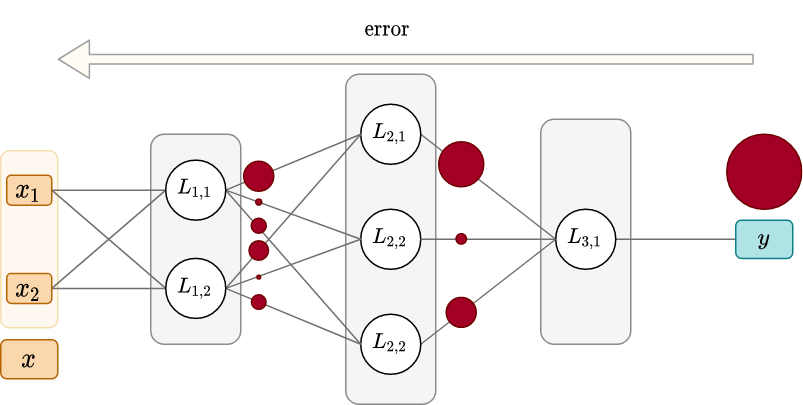
\includegraphics[width=14cm]{images/state-of-art/back-propagation/network_descent_gradient.png}
    \caption{Representation of the backpropagation algorithm.}
    \label{fig:basic_network}
\end{figure}

In this network, the error of each neuron is represented by red circles. The error calculated by the cost function is the largest error which indeed is the error of the output of the model. From that point, it will be backward propagated and computed which part of the error belongs to each neuron up to the first layer. For example, in the $L_2$ layer, the main neuron that has mismatched parameters is $L_{2,1}$. Likewise, this error is mainly due to the $L_{1,1}$ neuron. Therefore, it is logical to think that we should adjust neurons such as $L_{2,1}$ or $L_{1,1}$, however, leave neurons such as $L_{1,2}$ or $L_{2,2}$ as they are.
\newline
 
 The simplest neural network that can be constructed with a single hidden neuron and an output neuron is defined as follows:

\begin{figure}[H]
    \centering
    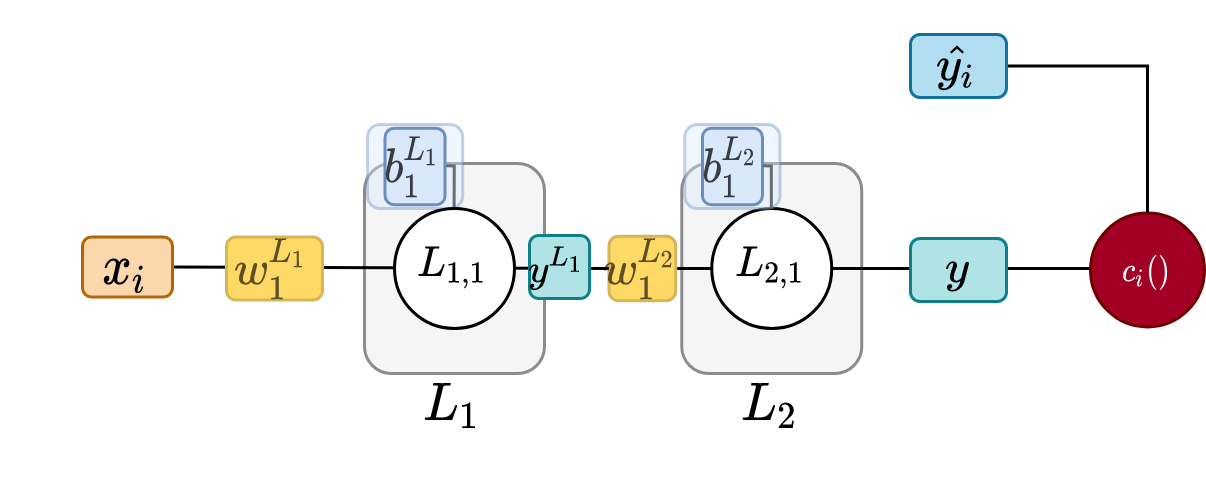
\includegraphics[width=12cm]{images/state-of-art/back-propagation/basic_network.png}
    \caption{Basic neural network.}
    \label{fig:basic_network}
\end{figure}

To perform the backpropagation algorithm, first the loss must be computed with the $c_i$ function. Then, the backpropagation algorithm will "distribute" the loss of the model to the previous layers (always starting with the last layer). This computation expresses how important the $W$ matrices are by indicating how much impact they have on the model. For example, if you change any value of $W_2$ in any way, you will be able to know how it affects the outcome of the model's prediction. Mathematically:

\begin{equation}
\begin{split}
    \frac{\partial c}{\partial w^{L_2}} &= \frac{\partial c(a(z^{L_2}))}{\partial w^{L_2}} \\
    \frac{\partial c}{\partial b^{L_2}} &= \frac{\partial c(a(z^{L_2}))}{\partial b^{L_2}} 
    \label{eqn:backpropagationsimplenetworklayer2}
\end{split}
\end{equation}

The numerator is a composition of functions and is basically the calculation of the forward-pass algorithm (see section \ref{feedforward}). To calculate the partial derivative of a composition of functions, it is necessary to use a calculation tool known as the chain rule.
\newline


An example to understand the chain rule would be the following. The Sun is known to be $100$ times larger than the Earth. The Earth is $4$ times larger than the Moon. Knowing these two relationships, we can tell how much the Sun is bigger than the Moon. To do this we simply multiply $100 \times 4 = 400$. The Sun is therefore $400$ times bigger than the Moon. Defining this problem with equations:
\begin{equation}
\begin{split}
    \frac{\partial T_{\text{Sun}}}{\partial T_{\text{Earth}}} = 100
    \qquad
    \frac{\partial T_{\text{Earth}}}{\partial T_{\text{Moon}}} = 4 \\
    \frac{\partial T_{\text{Sun}}}{\partial T_{\text{Moon}}} = \frac{\partial T_{\text{Sun}}}{\partial T_{\text{Earth}}} \cdot \frac{\partial T_{\text{Earth}}}{\partial T_{\text{Moon}}} = 400 \nonumber
\end{split}
\end{equation}


It is called the chain rule because it is chained in relation to the common data, in this case $T_\text{Earth}$ is the common part that on one side is in the denominator and on the other in the numerator. Therefore, to derive the composition of functions seen in equation \ref{eqn:backpropagationsimplenetworklayer2}, we simply have to multiply each of the intermediate derivatives. Recalling the equations of the forward-pass algorithm and the composition of functions to calculate the model error for the network shown in figure \ref{fig:basic_network}:


\begin{equation}
\begin{split}
    z^{L_2} = W^{L_2} \cdot y^{L_1} + b^{L_2}
    \qquad
    c(a^{L_2}(z^{L_2}))
\end{split}
\end{equation}

It is calculated how the error is propagated from the $L_2$ layer to the $L_1$ layer:

\begin{equation}
\begin{split}
     \frac{\partial c}{\partial w^{L_2}} &= \frac{\partial c}{\partial a^{L_2}} \cdot \frac{\partial a^{L_2}}{\partial z^{L_2}} \cdot \frac{\partial z^{L_2}}{\partial w^{L_2}} \\
     \frac{\partial c}{\partial b^{L_2}} &= \frac{\partial c}{\partial a^{L_2}} \cdot \frac{\partial a^{L_2}}{\partial z^{L_2}} \cdot \frac{\partial z^{L_2}}{\partial b^{L_2}}
\end{split}
 \label{eqn:backpropagationlayer2}
\end{equation}

These derivatives are easy to calculate and the explanation of each derivative would be as follows:


\begin{itemize}
\item First derivative. Derived from the activation function with respect to cost:

\begin{equation}
    \frac{\partial c}{\partial a^{L_2}}
\end{equation}

How does the cost of the network (it is the last layer) vary when the output of the network activation function is varied? In other words, the derivative of the cost function is calculated with respect to the output of the neural network. It is therefore necessary to know the derivative of the cost function used.

\item Second derivative. Derived from activation with respect to $z$:
\begin{equation}
    \frac{\partial a^{L_2}}{\partial z^{L_2}}
\end{equation}


It tries to reflect how the output of the neuron varies when the weighted sum of the neuron is varied. The derivative to be used is the derivative of the activation function. Derived from the sum of the weighted values of the weights and biases.

\item Third derivative: Derived from $z$ with respect to the parameters:
\begin{align*}
    \frac{\partial z^{L_2}}{\partial w^{L_2}} && \frac{\partial z^{L_2}}{\partial b^{L_2}}
\end{align*}

It indicates how the weighted sum $z$ varies with respect to a variation in the parameters. Parameter $b$ is an independent value so its derivative is a constant equal to 1. On the other hand, the derivative $\frac{\partial z^{L_2}}{\partial w^{L_2}}$ depends on the previous layer.


\begin{align*}
    \frac{\partial z^{L_2}}{\partial w^{L_2}} = a^{L_1} && \frac{\partial z^{L_2}}{\partial b^{L_2}} = 1
\end{align*}

\end{itemize}

Based on this definition, the first and second derivatives can be combined into one:

\begin{equation}
     \frac{\partial c}{\partial a^{L_2}} \cdot \frac{\partial a^{L_2}}{\partial z^{L_2}} = \frac{\partial c}{\partial z^{L_2}}
\end{equation}

This derivative indicates the degree to which the error is modified when there is a change in the error when there is a small change in the sum of the neurons in the layer. If the value is large it means that a small change in any of the neurons in the layers in the $z$ value will be reflected in the result of the model. On the contrary, if the value is small, a large change in any of the neurons in the $z$ value of will not affect the final result. In summary, this derivative shows how the layer (or some neuron in particular since it is a vector) affects the final result and therefore the error of the network and in that way the algorithm of the descent of the gradient will modify the parameters to be able to obtain the best possible result. This derivative is also known as the layer error and is represented by $\delta$:

\begin{equation}
    \frac{\partial c}{\partial a^{L_2}} \cdot \frac{\partial a^{L_2}}{\partial z^{L_2}} = \frac{\partial c}{\partial z^{L_2}} = \delta^{L_2}
\end{equation}

With this new definition, equation \ref{eqn:backpropagationlayer2} can be rewritten as follows:

\begin{equation}
\begin{split}
     \frac{\partial c}{\partial w^{L_2}} &= \frac{\partial c}{\partial a^{L_2}} \cdot \frac{\partial a^{L_2}}{\partial z^{L_2}} \cdot \frac{\partial z^{L_2}}{\partial w^{L_2}} \\ &= \delta^{L_2} \cdot \frac{\partial z^{L_2}}{\partial w^{L_2}} = \delta^{L_2} \cdot a^{L_1}
\end{split}
\label{eqn:backpropagation_b}
\end{equation}

\begin{equation}
\begin{split}
     \frac{\partial c}{\partial b^{L_2}} &= \frac{\partial c}{\partial a^{L_2}} \cdot \frac{\partial a^{L_2}}{\partial z^{L_2}} \cdot \frac{\partial z^{L_2}}{\partial b^{L_2}} \\ &= \delta^{L_2} \cdot \frac{\partial z^{L_2}}{\partial b^{L_2}} = \delta^{L_2} \cdot 1
\end{split}
\label{eqn:backpropagation_w}
\end{equation}

But the model does not only depend on the second layer and $W_2$, it also depends on the first layer and $W_1$. This is where the beauty of the backpropagation algorithm comes in. The error can be backpropagated in a similar way using the same reasoning. First the composition of functions is shown:

\begin{equation}
\begin{split}
    \frac{\partial c}{\partial w^{L_1}} &= \frac{\partial c(a(z^{L_2}(a(z^{L_1}))))}{\partial w^{L_2}} \\
    \frac{\partial c}{\partial b^{L_1}} &= \frac{\partial c(a(z^{L_2}(a(z^{L_1}))))}{\partial b^{L_2}} 
    \label{eqn:backpropagationsimplenetworklayer2}
\end{split}
\end{equation}

Using the chain rule it is divided into different parts:

\begin{equation}
\begin{split}
     \frac{\partial c}{\partial w^{L_1}} &= \frac{\partial c}{\partial a^{L_2}} \cdot \frac{\partial a^{L_2}}{\partial z^{L_2}} \cdot \frac{\partial z^{L_2}}{\partial a^{L_1}} \cdot \frac{\partial a^{L_1}}{\partial z^{L_1}} \cdot \frac{\partial z^{L_1}}{\partial x} \\
     \frac{\partial c}{\partial b^{L_1}} &= \frac{\partial c}{\partial a^{L_2}} \cdot \frac{\partial a^{L_2}}{\partial z^{L_2}} \cdot \frac{\partial z^{L_2}}{\partial a^{L_1}} \cdot \frac{\partial a^{L_1}}{\partial z^{L_1}} \cdot \frac{\partial z^{L_1}}{\partial 1} \\
\end{split}
 \label{eqn:backpropagationlayer1}
\end{equation}

In fact, of the $6$ derivatives shown, only one would need to be calculated. The derivatives $\frac{\partial c}{\partial a^{L_2}} \cdot \frac{\partial a^{L_2}}{\partial z^{L_2}} $ have already been calculated and are equal to $\delta^{L_2}$. As for the derivative $\frac{\partial z^{L_1}}{\partial x}$ If you want to use the first layer, simply get the result of the previous layer or use $x$ if it is the first layer as it is in this case. The derivative $\frac{\partial z^{L_1}}{\partial 1}$ is a constant value so nothing happens. Finally, the derivative $\frac{\partial a^{L_1}}{\partial z^{L_1}}$ is simply the derivative of the activation function of that layer. This is why in section \ref{activationfunction} it was explained that it is better to use a single activation function for the whole layer and thus facilitate the calculations.
\newline

The only derivative that remains to be explained is $\frac{\partial z^{L_2}}{\partial a^{L_1}}$ the one that expresses how the weighted sum of a layer varies when the input vector of that layer is varied. The calculation of this derivative is simply the matrix of parameters $W^{L_1}$ that connects both layers. Basically, this derivative moves the error from layer $L_2$ to layer $L_1$ distributing the error according to the weightings of the connections. As it was done with the previous layer, with this layer it is also possible to define the imputed error:


\begin{equation}
   \frac{\partial c}{\partial a^{L_1}} = \frac{\partial c}{\partial a^{L_2}} \cdot \frac{\partial a^{L_2}}{\partial z^{L_2}} \cdot \frac{\partial z^{L_2}}{\partial a^{L_1}} \cdot \frac{\partial a^{L_1}}{\partial z^{L_1}} = \delta^{L_1}
\end{equation}

Therefore, equation \ref{eqn:backpropagationlayer1} would look like this:

\begin{equation}
\begin{split}
     \frac{\partial c}{\partial w^{L_1}} &= \delta^{L_1} \cdot \frac{\partial z^{L_1}}{\partial x} \\
     \frac{\partial c}{\partial b^{L_1}} &= \delta^{L_1} \frac{\partial z^{L_1}}{\partial 1} \\
\end{split}
\end{equation}

In summary, it has been possible to explain how to propagate the error to any layer of the network and calculate the derivative with respect to the parameters with the following equations:

\begin{equation}
\begin{split}
     \frac{\partial c}{\partial w^{L_1}} &= \delta^{L_1} \cdot \frac{\partial z^{L_1}}{\partial x} \\
     \frac{\partial c}{\partial b^{L_1}} &= \delta^{L_1} \\
     \frac{\partial c}{\partial w^{L_2}} &= \delta^{L_2} \cdot \frac{\partial z^{L_2}}{\partial a^{L_1}} \\
     \frac{\partial c}{\partial b^{L_2}} &= \delta^{L_2}
\end{split}
\end{equation}

In view of the backpropagation algorithm for the network defined in figure \ref{fig:basic_network}, the algorithm is divided into different steps:
\begin{enumerate}
    
    \item Initialise index to know in the layer to be computed
    \begin{equation}
    \begin{split}
        i=l; l > 0 \\
    \end{split}
    \end{equation}
    
    
    \item \label{alg:backpropagation_loop} Calculation of the imputed error of the layer:
    \begin{enumerate}
        \item If $i=l$:
        \begin{equation}
        \delta^{L_i} = \frac{\partial c}{\partial a^{L_i}} \cdot \frac{\partial a^{L_i}}{\partial z^{L_i}}
        \end{equation}
        
        \item \acrshort{ioc}:
        
        \begin{equation}
        \delta^{L_i} = \delta^{L_{i+1}} \cdot \frac{z^{L_{i+1}}}{\partial a^{L_i}} \cdot \frac{\partial a^{L_i}}{\partial z^{L_i}}
        \end{equation}
    \end{enumerate}
    
    \item 3.	Calculation of derivatives on parameters $b$ and $W$:
    \begin{enumerate}
        \item Calculation on $b$:
        \begin{equation}
        \frac{\partial c}{\partial b^{L_i}} = \delta^{L_{i}}
        \end{equation}
        
        \item Calculation on $w$:
        \begin{enumerate}
            \item If $i=1$:
                \begin{equation}
                \frac{\partial c}{\partial w^{L_i}} = \delta^{L_{i}} \cdot x
                \end{equation}
            \item e.o.c:
                \begin{equation}
                \frac{\partial c}{\partial w^{L_i}} = \delta^{L_{i}} \cdot a^{L_{i-1}}
                \end{equation}
        \end{enumerate}
    \end{enumerate}
    
    \item Update the index:
    \begin{equation}
    i = i-1
    \end{equation}
    
    \item If $i>0$ go back to step \ref{alg:backpropagation_loop}
\end{enumerate}

With this, it has been possible to obtain the partial derivatives of each layer of the network so that it will be possible to calculate the new $W$ matrices using the method of the descent of the gradient explained in section \ref{minimizing-error}.